\section{Logic Gates}

The basic building blocks of computers are called \emph{gates}. Their only function is to report, with some yes-or-no electrical output, the result of their circuit following some input from somewhere else in the circuit. The way to understand how gates make decisions is called ``Boolean Algebra", but really it's a fairly simple set of decisions that get strung together in useful ways.

\subsection*{Boolean Logic}

Boolean logic is the sort of decision making and answers that computers use. You can use it too, of course, and it will help you learn to program computers. The answer to every question in Boolean logic is either ``yes'' or ``no'' -- ``true'' or ``false''. In computers, that's a one or a zero, of course.   Every operation (decision) is composed of a set of operations: \emph{and}, \emph{or}, and \emph{not}. A British man named George Boole introduced these ideas to the world in 1847\footnote{
\emph{The Mathematical Analysis of Logic} (1847), and \emph{An Investigation of the Laws of Thought} (1854). For more, see his {\color{webblue}\href{https://en.wikipedia.org/wiki/George_Boole}{Wikipedia entry}}.}. He did not realize he was laying the foundations for computing, but 50 years later another very important mathematician, Claude Shannon, understood that Boole's system for understanding decisions could be used to design electronic circuits\footnote{Shannon, Claude E. 1938. ``A Symbolic Analysis of Relay and Switching Circuits". \emph{Trans. AIEE.} 57 (12): 713--723.}. 

It may be helpful to see some of the logic and operations (decisions) made in a graphical form, looking at the overlap between circles, or between a circle and its surrounding area.

% Draw Venn diagrams to graphically demonstrate OR, AND, and NOT.
\begin{figure}[!h]
\begin{center}
% Definition of circles and square
\def\firstcircle{(0,0) circle (1.5cm)}
\def\secondcircle{(0:2cm) circle (1.5cm)}
\def\firstsquare{(-1.6,-1.6) rectangle (1.6,1.6)}

% Set colors
\colorlet{circle edge}{blue!50}
\colorlet{circle area}{blue!20}
\colorlet{rectangle edge}{blue!50}
\colorlet{rectangle area}{blue!20}

\tikzset{filled/.style={fill=circle area, draw=circle edge, thick},
    outline/.style={draw=circle edge, thick}}
\setlength{\parskip}{5mm}


\begin{tabular}{p{2.25in} p{2.25in} p{2.25in}}

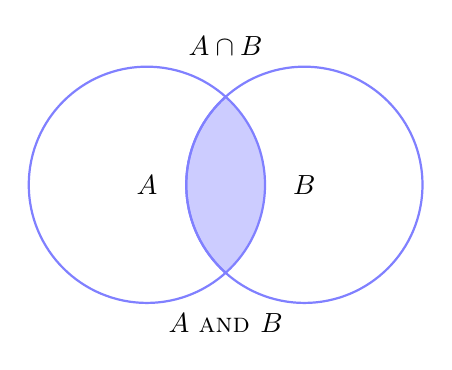
\begin{tikzpicture}

	\begin{scope}
        \clip \firstcircle;
        \fill[filled] \secondcircle;
    \end{scope}

    \draw[outline] \firstcircle node {$A$};
    \draw[outline] \secondcircle node {$B$};
    \node[anchor=south] at (current bounding box.north) {$A \cap B$};
	\node[anchor=north] at (current bounding box.south) {$A$ \sc{and} $B$};

\end{tikzpicture}

&

% Set A or B
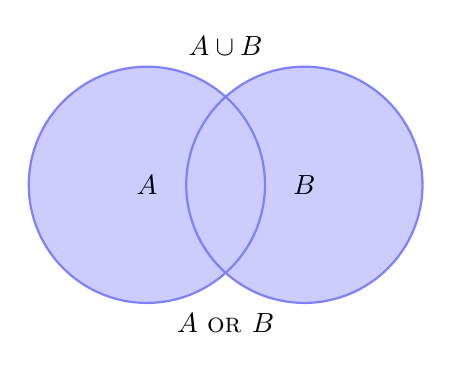
\begin{tikzpicture}

    \draw[filled] \firstcircle node {$A$}
                  \secondcircle node {$B$};
    \node[anchor=south] at (current bounding box.north) {$A \cup B$};
	\node[anchor=north] at (current bounding box.south) {$A$ \sc{or} $B$};

\end{tikzpicture}

&

% NOT A

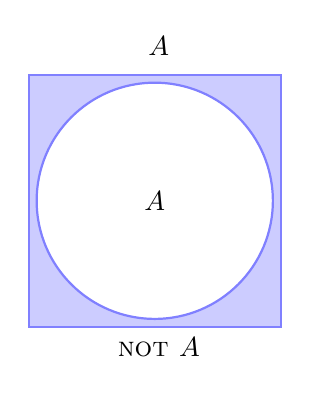
\begin{tikzpicture}

	\filldraw[blue!20,even odd rule] \firstsquare \firstcircle;
	\draw[outline] \firstcircle node{$A$};
	\draw[outline] \firstsquare node{};
	\node[anchor=south] at (current bounding box.north) {$\thicksim A$};
	\node[anchor=north] at (current bounding box.south) {\sc{not} $A$};

\end{tikzpicture}

\\

\end{tabular}

\caption{A graphic representing {\sc{and}}, {\sc{or}}, and {\sc{not}} with overlapping circles.}
\end{center}
\label{fig:vennlogic}
\end{figure}


Also note: more complex decisions can be made by combining these operations: NOT $+$ AND, for instance). 


\subsection*{The OR Gate}

OR gates take two inputs and provide a ``yes'' if line 1 OR line 2 are equal to 1 -- that is, if either line has a voltage level above zero.

\medskip
\begin{center}

\begin{tabular}{p{2.3in} p{3.7in} }
\hline\\[\negsep]
The symbol for an OR gate is:

\vspace{0.25in}

\begin{circuitikz}
	\draw(0,0)
	node[american or port](orgate){}
	(orgate.in 1) node [left](){{\color{red}$INPUT~A$}}
	(orgate.in 2) node [left](){{\color{red}$INPUT~B$}}
	(orgate.out) node [right](){{\color{red}$OUT$}}
;
\end{circuitikz}

&

\centering

The ``Truth Table" (how they behave) is: 
\vspace{0.15in}

\begin{tabular}{ll | c}
\multicolumn{3}{c}{\textbf{OR Gate }}\\
\multicolumn{3}{c}{\textbf{Truth Table}}\\
\hline\\[\negsep]
\textbf{A} & \textbf{B} & \textbf{OUT}\\
\hline
0 & 0 & 0  \\
1 & 0 & 1  \\
0 & 1 & 1  \\
1 & 1 & 1  \\
\hline
\end{tabular}
\\
\tabularnewline
\hline\\[\negsep]
\end{tabular}

\end{center}
\bigskip

\noindent OR gates are very simple. They are so simple that transistors are not even needed, though they certainly can be used.

\begin{figure}[!h]
\begin{center}
\begin{circuitikz}

\draw 
% IN nodes:
	(0,5) node[ocirc](ina) {}
	(0,5) node[left] {{\color{red}$INPUT~A$}} % INPUT A label
	(0,3) node[ocirc](inb) {}
	(0,3) node[left] {{\color{red}$INPUT~B$}} % INPUT B label


% OUT node:
	(4.5,3) node[ocirc](out){} 
	(4.5,3) node[right] {{\color{red}$OUT$}} % OUT label
	(3,3) |- (out)
	(3,3) node[circ](outjoint){}

%  GND:
    (3,0) node[ground](ground){}
    
% Diodes:
	(ina) to [Do, l^=$D_1$] (2,5)
	(inb) to [Do, l^=$D_2$] (2,3) 

% Resistor:
	(3,3) to [R, l^=$R_1$] (ground)

% Nets:
		(2,4) node[circ](diodemerge){}
		(2,5) to (diodemerge)
		(2,3) to (diodemerge)
		(diodemerge) to (3,4)
		(3,4) to (outjoint)

;
\end{circuitikz}

\caption{A very simple OR gate schematic. Diodes conduct electricity only in the ``forward'' direction. So Input A cannot affect Input B. But either way, if there is a signal on Input A or on Input B, OUT will carry a voltage (and therefore, a ``1''). Diode \emph{propagation delay} (how much time the signal takes to cross through the diode) is slower than transistors, meaning transistorized circuits run faster.}
\label{fig:diodeorgate}
\end{center}
\end{figure}

\stbox{\emph{Experiment:} Wire up an OR gate on a breadboard, like the one seen in the cover image. Use LEDs as indicators for Input A, Input B, and OUT. Feel free to use diodes, but using transistors is pretty easy. It's best to use N-type transistors as switches for each LED and for the OR-output LED.}

\begin{figure}[!ht]
\begin{center}
\begin{circuitikz}

\draw 
% IN nodes:
	(3,6) node[ocirc](ina) {}
	(3,6) node[left] {{\color{red}$INPUT~A$}} % INPUT A label
	(3,3) node[ocirc](inb) {}
	(3,3) node[left] {{\color{red}$INPUT~B$}} % INPUT B label


% OUT node:
	(8.5,2) node[ocirc](out){} 
	(8.5,2) node[right] {{\color{red}$OUT$}} % OUT label
	(6.0,2) |- (out)
	(6.0,2) node[circ](outjoint){}

% 2 Transistors:
	(7,6) node[npn](Q1){$Q_1$}
	(6,3) node[npn](Q2){$Q_2$}

% Vcc and GND:
	(7,7.5) node[vcc](vcc){$V_{cc}$}
	(6,4.25) node[vcc](vcc1){$V_{cc}$}
    (6,0) node[ground](ground){}
    
% Resistors:
	(ina) to [R, l^=$R_1$] (5,6)
	(5,6) |- (Q1.B)
	(inb) to [R, l^=$R_2$] (Q2.B) 
	(Q2.E) to [R, l^=$R_3$] (ground)

% Nets:
	(Q1.E) |- (7,4.0)
	(7,4.0) |- (7,2)
	(7,2) node[circ](){}
	
	(vcc) |- (Q1.C)
	(vcc1) |- (Q2.C)
;
\end{circuitikz}
\caption{A simple transistor-based OR gate. Transistors are better than diodes in this application because transistors amplify (or at least do not degrade) signals, while diodes lose half a volt or more.  In this schematic, each transistor acts as an independent switch for the output -- either switch pushes OUT to high.}
\label{fig:npnorgate}
\end{center}
\end{figure}

\begin{figure}[!ht]
\begin{center}
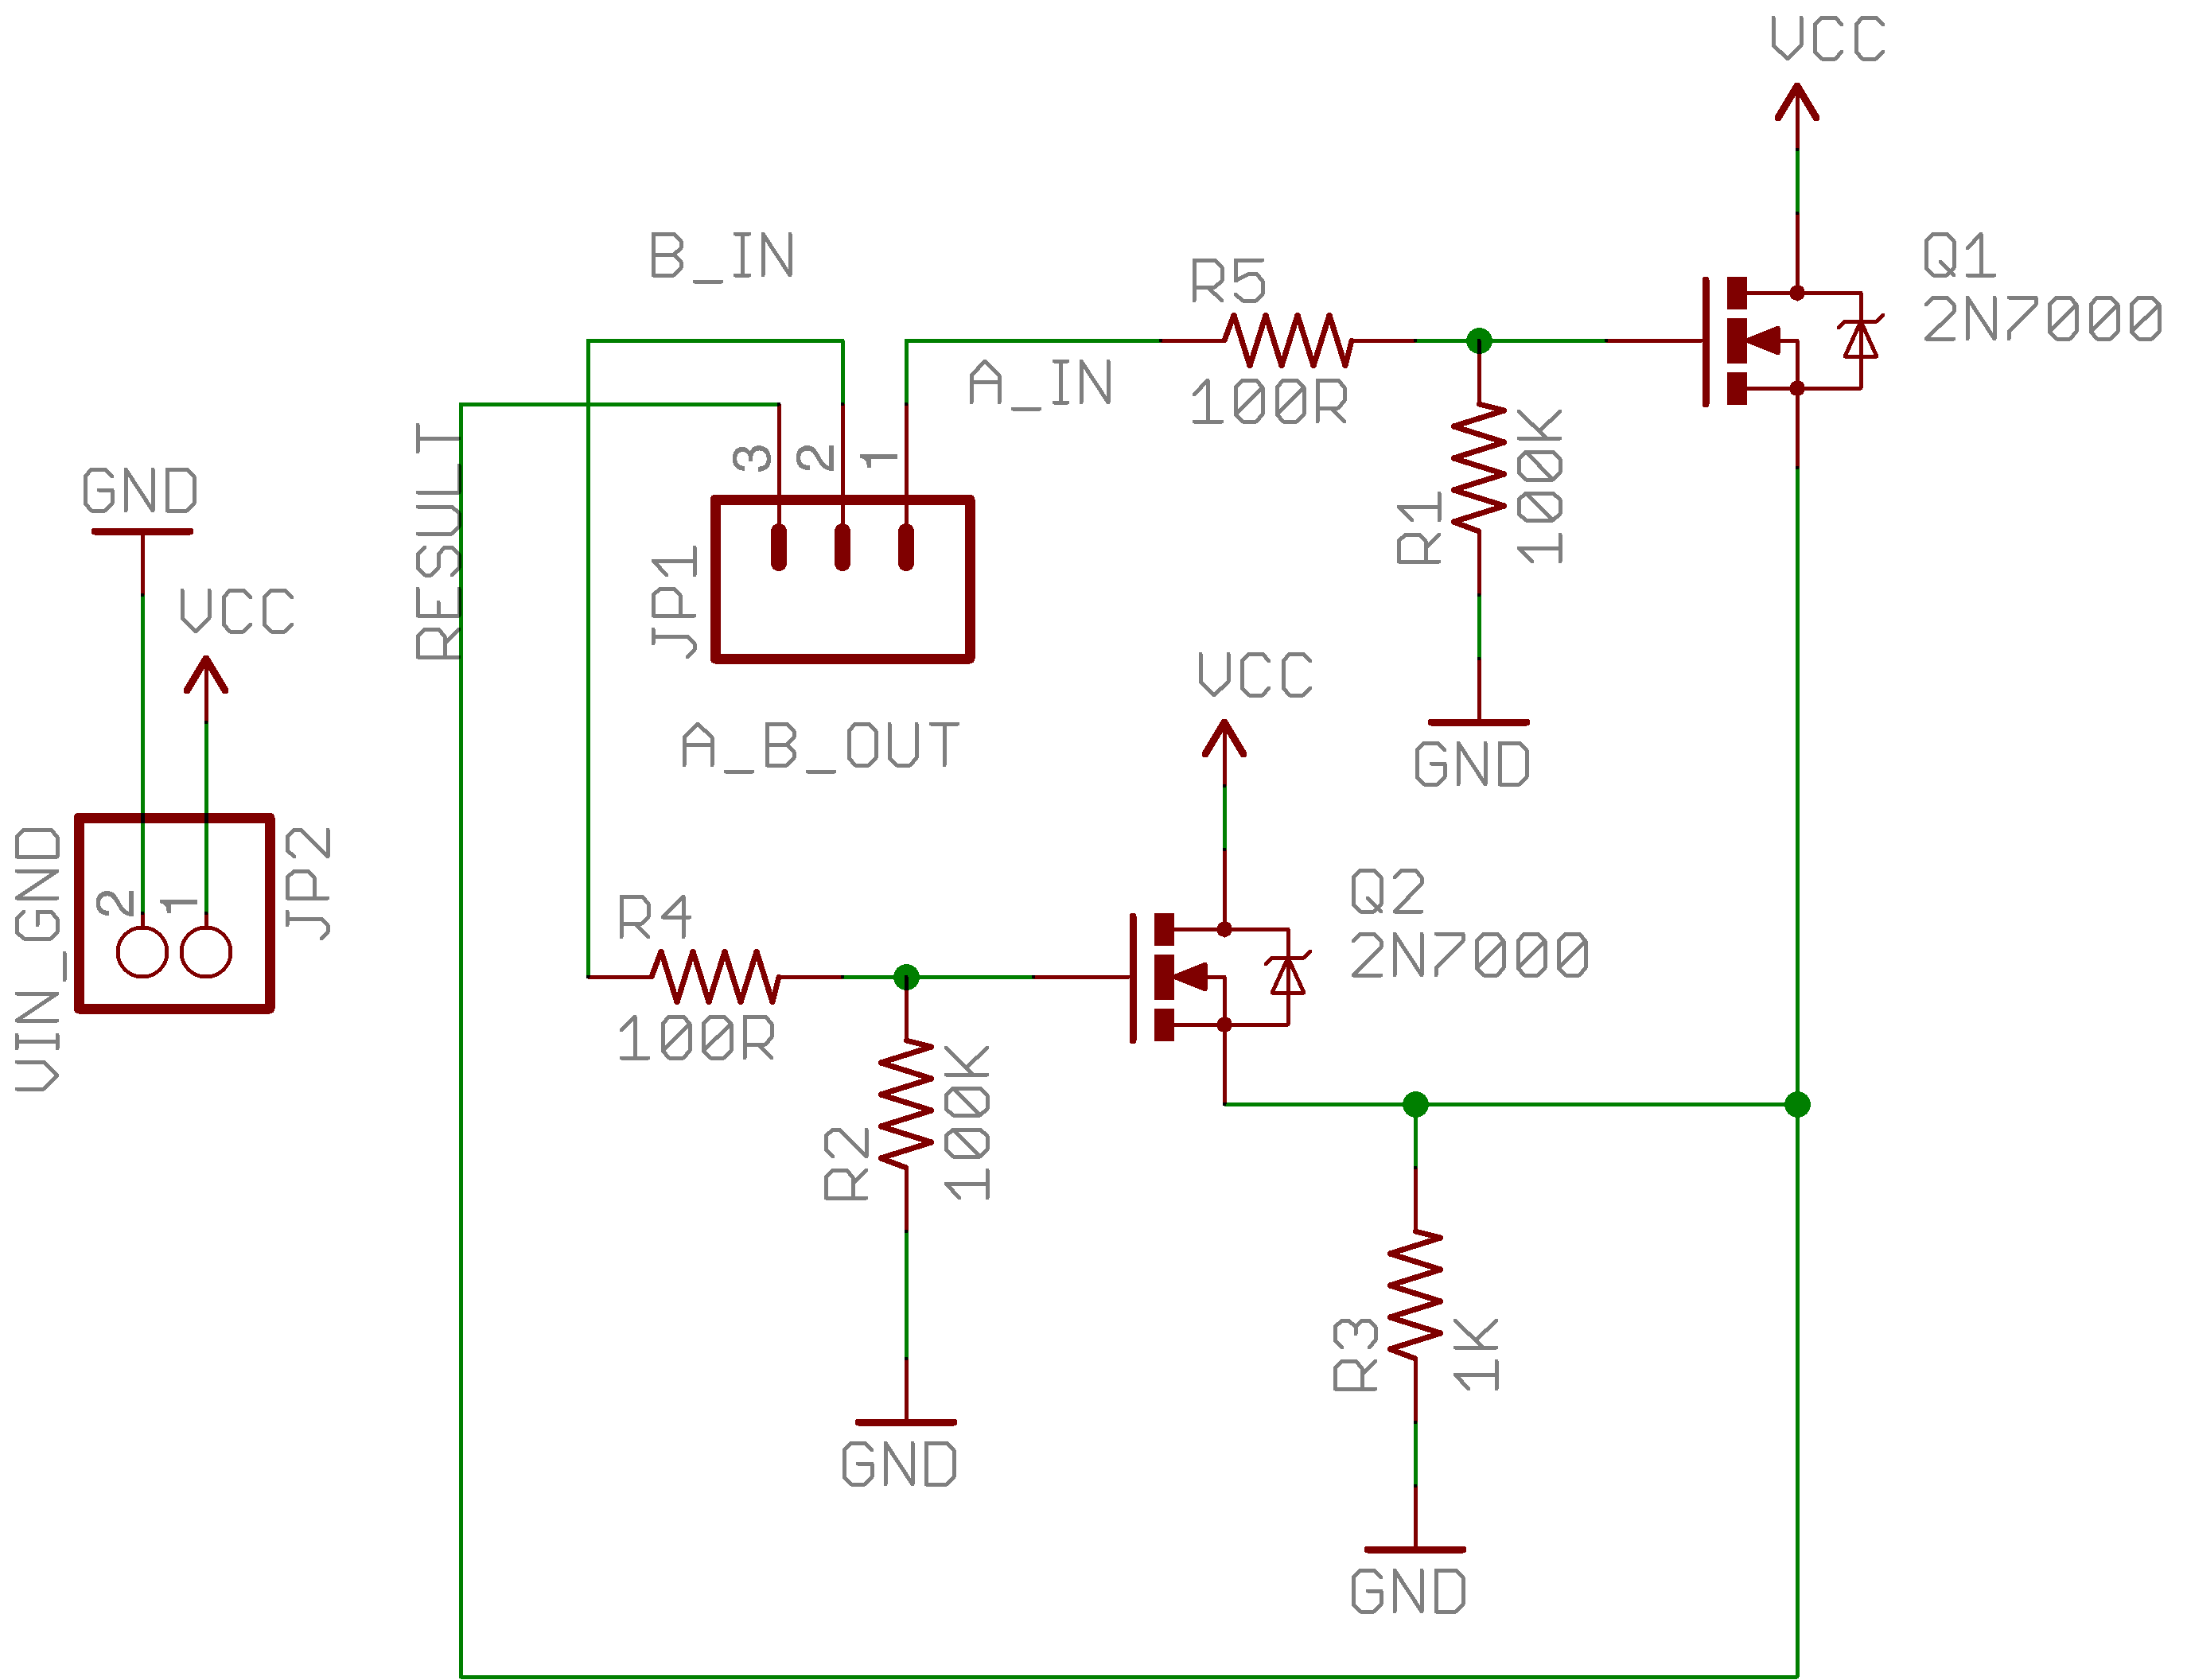
\includegraphics[scale=1.25]{orgateschembetter.png}
\caption{A schematic from a real circuit design program showing a practical, real implementation of the idealized schematic in Figure \ref{fig:npnorgate}. The wires connecting components are the green lines. Mostly there are more resistors to help keep the transistors behaving well. For instance, the 100K resistors make sure the transistors are always at a low logic level (zero volts) when the inputs are `off'.}
\label{fig:orgateeagleschematic}
\end{center}
\end{figure}




\begin{figure}[!hb]
\begin{center}
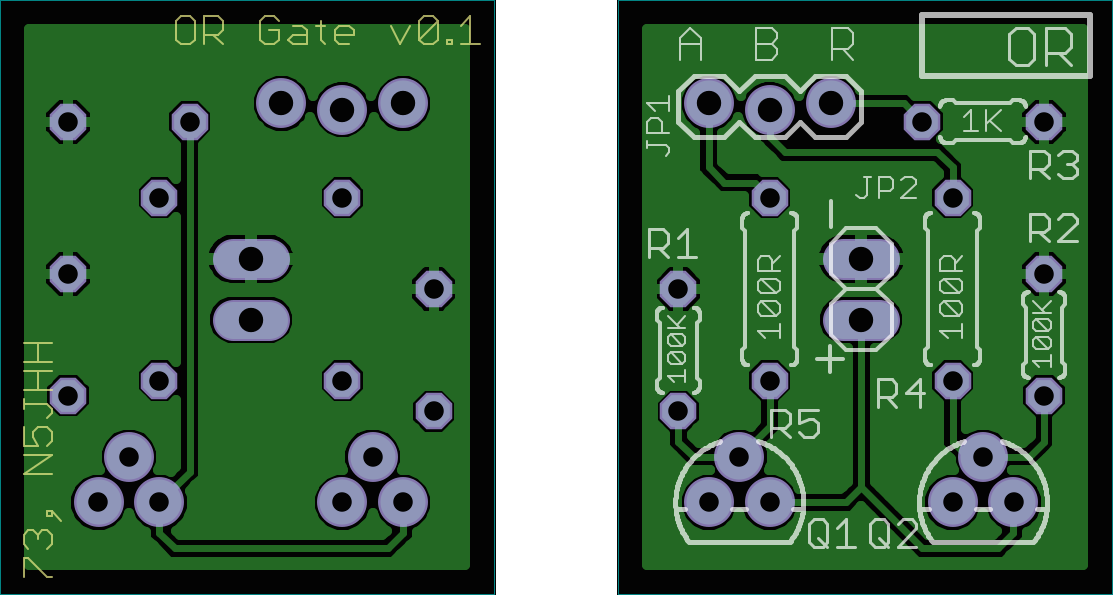
\includegraphics[scale=0.25]{trimmedorgate.png}
\caption{A circuit board designed using the above OR gate schematic. You can solder these without much trouble. You can see the top and bottom of the board here, but all components go on the top. However, both top and bottom have \emph{traces}, that carry electricity instead of using loose/floppy wires. The larger resistors are the lowest value (they're just there to make the transistors behave a little better): 100R means ``100 Ohms''. The smaller resistors are either 100,000 Ohms (that is, 100K Ohms) or 1,000 Ohms (1K Ohms). The OR gate takes two \emph{inputs}, A and B, and produces one \emph{result}, R.}
\label{fig:orgatepcbs}
\end{center}
\end{figure}





\clearpage
\newpage

\subsection*{The AND Gate}

AND gates take two inputs and provide a ``yes'' (a one, or a ``logic high" signal) only if both line 1 AND line 2 are equal to 1.

\medskip
\begin{center}

\begin{tabular}{p{2.3in} p{3.7in} }
\hline\\[\negsep]

The symbol for an AND gate is:

\vspace{0.25in}

\begin{circuitikz}
	\draw(0,0)
	node[american and port](andgate){}
	(andgate.in 1) node [left](){{\color{red}$INPUT~A$}}
	(andgate.in 2) node [left](){{\color{red}$INPUT~B$}}
	(andgate.out) node [right](){{\color{red}$OUT$}};

\end{circuitikz}

&

\centering

The ``Truth Table" (how they behave) is: 
\vspace{0.15in}

\begin{tabular}{ll | c}
\multicolumn{3}{c}{\textbf{AND Gate }}\\
\multicolumn{3}{c}{\textbf{Truth Table}}\\
\hline\\[\negsep]
\textbf{A} & \textbf{B} & \textbf{OUT}\\
\hline
0 & 0 & 0  \\
1 & 0 & 0  \\
0 & 1 & 0  \\
1 & 1 & 1  \\
\hline
\end{tabular}
\\
\tabularnewline

\hline\\[\negsep]

\end{tabular}
\end{center}

\bigskip


There are much more complicated AND gates, but see below for an easy-to-understand example (and it totally works). Remember that transistors act like switches: the \emph{gate} acts like the switch that opens up the flow of electricity from the \emph{source} to the \emph{drain}. Look at the schematic in Figure \ref{fig:simpleandgate} -- note that the drain of the top transistor ($Q_1$) flows into the source of the other transistor ($Q_2$), meaning that even if $Q_2$ is turned on, it may not necessarily start carrying electricity (because $Q_1$ may not allow the electricity from $V_{cc}$ to pass through). Thus, both gate 1 AND gate 2 have to be turned on in order to see voltage at the output.

\bigskip

\begin{figure}[!ht]
\begin{center}
\begin{circuitikz}

\draw 
% IN nodes:
	(3,5) node[ocirc](ina) {}
	(3,5) node[left] {{\color{red}$INPUT~A$}} % INPUT A label
	(3,3) node[ocirc](inb) {}
	(3,3) node[left] {{\color{red}$INPUT~B$}} % INPUT B label


% OUT node:
	(7.5,2) node[ocirc](out){} 
	(7.5,2) node[right] {{\color{red}$OUT$}} % OUT label
	(6,2) |- (out)
	(6,2) node[circ](outjoint){}

% 2 Transistors:
	(6,5) node[npn](Q1){$Q_1$}
	(6,3) node[npn](Q2){$Q_2$}

% Vcc and GND:
	(6,6.5) node[vcc](vcc){$V_{cc}$}
    (6,0) node[ground](ground){}
    
% Resistors:
	(ina) to [R, l^=$R_1$] (Q1.B)
	(inb) to [R, l^=$R_2$] (Q2.B) 
	(Q2.E) to [R, l^=$R_3$] (ground) 

% Nets:
	(Q1.E) to (Q2.C)
	(vcc) to (Q1.C)
;
\end{circuitikz}

\caption{A simple AND gate schematic. When Input A is a zero, no current flows into the ``collector" (voltage input wire) of Transistor 2. When Input B is zero, no current can flow to OUT, regardless of whether Input A is 0 or 1. Only when Input A is 1 (current can flow past Q1) and when Input B is 1 (current is available to Q2, and Q2 is turned ``on'', allowing current to pass) does OUT go ``high". $R_3$ prevents too much current from flowing to ground, and is not strictly necessary in all gates, but is included here because it is common to see them. $R_1$ and $R_2$ should be about 100 ohms. $R_3$ should be about 100K ohms. This design is just for demonstration.}
\label{fig:simpleandgate}
\end{center}
\end{figure}


\begin{figure}[!ht]
\begin{center}
\fbox{
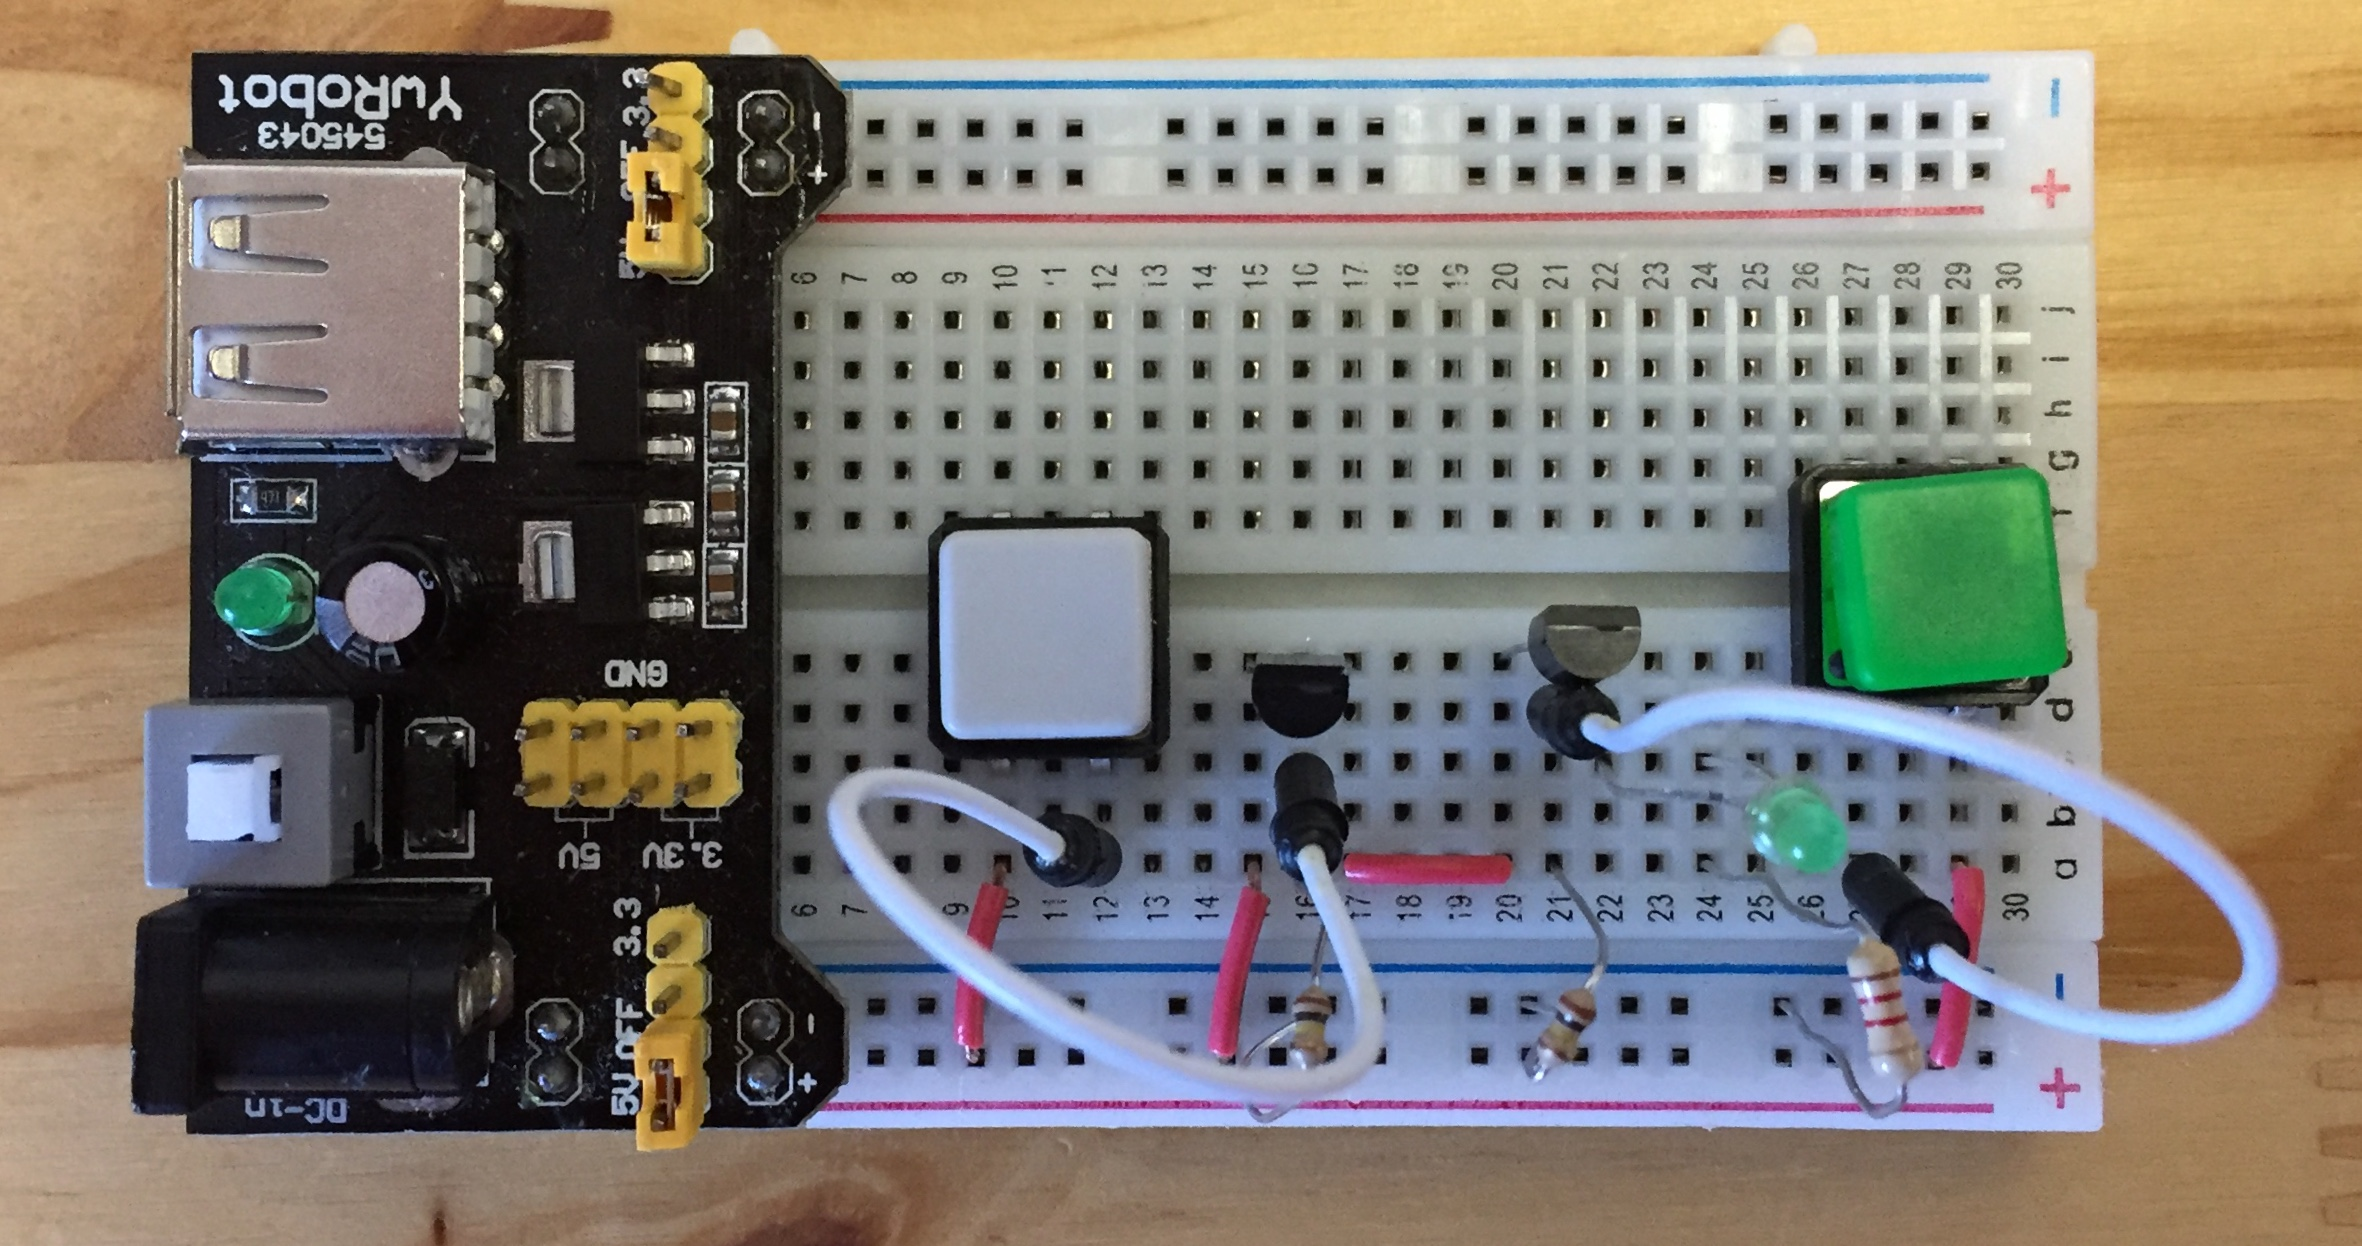
\includegraphics[scale=0.14]{andgatebreadboard.jpg}
}
\medskip

A single AND gate on a solderless breadboard. The transistor on the left, controlled by the gray button, makes electricity available to the input of the second transistor, controlled by the green button. Only if both transistors are ``on'' (that is, A \emph{and} B are passing electricity) will the LED light up. Using this picture, wire up an AND gate on a breadboard with N-type transistors. Use LEDs as indicators for Input A, Input B, and the result.
\end{center}
\end{figure}





\begin{figure}[!ht]
\begin{center}
\includegraphics[scale=0.25]{andgate.png}
\caption{A circuit board designed using the above AND gate schematic, though with two 100K pull-down resistors also implemented (these guarantee the transistor's gate are reliably held at 0 volts instead of allowed to \emph{float}, until either of the inputs goes high (that is, pushes some voltage into the transistor gate). The pull-down resistors are important practically, but they do not appear in this circuit diagram for simplicity. This board looks almost exactly like the OR gate, but the wiring is different! Also, you can see both the front and back sides of the circuit board in this image. The AND gate takes two \emph{inputs}, A and B, and produces one \emph{result}, R.}
\end{center}
\label{fig:andgate}
\end{figure}


\clearpage
\newpage

\subsection*{The NOT Gate}

NOT gates take one input and reverse the value of that input. So a 1 becomes a 0, or vice versa. Also note this is the \emph{complement} of the input value, as seen above.

\medskip
\begin{center}

\begin{tabular}{p{2.3in} p{3.7in} }
\hline\\[\negsep]

The symbol for a NOT gate is:
\vspace{0.25in}

\begin{circuitikz}
	\draw(0,-0.5)
	node[american not port](notgate){}
	(notgate.in) node [left](){{\color{red}$INPUT$}}
	(notgate.out) node [right](){{\color{red}$OUT$}}
;
\end{circuitikz}

&

\centering

The ``Truth Table" (how they behave) is: 
\vspace{0.15in}

\begin{tabular}{l | c}
\multicolumn{2}{c}{\textbf{NOT Gate }}\\
\multicolumn{2}{c}{\textbf{Truth Table}}\\
\hline\\[\negsep]
\textbf{IN} & \textbf{OUT}\\
\hline
0 & 1 \\
1 & 0  \\
\hline
\end{tabular}
\\
\tabularnewline

\hline\\[\negsep]

\end{tabular}
\end{center}

\bigskip

A simple NOT circuit is easy to understand, though this example is not how NOT gates are actually implemented, because of the poor efficiency (and wasted energy turns into heat, which then has to be cooled somehow; it is better to not make the heat in the first place).

\begin{figure}[!h]
\begin{center}
\begin{circuitikz}

\draw 
% IN node:
	(1,3) node[ocirc](in) {}
	(1,3) node[left] {{\color{red}$IN$}} % IN label

% OUT node:
	(6.0,4) node[ocirc](out){} 
	(6.25,4) node[right] {{\color{red}$OUT$}} % OUT label

	(4,4) node[circ](){}

% The Transistor:
	(4,3) node[npn](Q1){}
	(4,2.75) node[right]{$Q_1$}

% Vcc and GND:
	(4,6.5) node[vcc](vcc){$V_{cc}$}
    (4,2) node[ground](ground){}
    
% Resistors:
	(1,3) to [R, l^=$R_1$] (3.5,3)
	(4,6) to [R, l^=$R_2$ ](4,4.5)


% Nets:
	(Q1.E) to (ground)
	(Q1.C) to (4,4.5)
	(4,6) to (vcc)
	(4,4) to (out)

;
\end{circuitikz}

\caption{A very simple NOT gate schematic. When IN is logic low (off), electricity cannot pass through to the ground, and so it is available at the OUT terminal. That means OUT is a 1. When IN is carrying current, the transistor opens up and electricity starts flowing to ground -- the ``path of least resistance''. Then, because $R_3$ provides a little resistance, electricity flows to ground instead of OUT, meaning OUT has a very, very low voltage available -- making it a zero.}
\label{fig:simplenot}
\end{center}
\end{figure}


\begin{figure}[!ht]
\begin{center}
\begin{circuitikz}

\draw 
	(0,4.0) node[ocirc](in) {} % IN node
	(0,4.0) node[left] {{\color{red}$IN$}} % IN label
	
	(8.5,4) node[ocirc](out){} % OUT node
	(8.75,4) node[right] {{\color{red}$OUT$}} % OUT label
	(7,4) |- (out)
	(7,4) node[circ](){}

% Vdd:
	(7,7.5) node[vcc](vin){}
    (6.5,7.5) node[above] {$V_{in}$} % Vin

% GND
    (7,0) node[ground](ground){}
%   (7.75,0.5) node[below] {{\color{red}$GND$}} % GND

% P-type FET
	(7,5) node[pmos, emptycircle, xscale=1](Q1){}
	(7.5,5.0) node[above]{$Q_1$}

% N-type FET
	(7,3) node[nmos, rotate=0](Q2){}
	(7.5,2.5) node[above]{$Q_2$}

% Resistors:
	(5,0) to [R, l^=$R_1$](5,3)
	(Q2.S) to [R, -*, l^=$R_2$](ground) 
	(in) to [R, -*, l^=$R_3$](3,4)
	(5,7) to [R, l^=$R_4$](5,5)

% Silicon Diodes: (1N4148)
	(3,5) to [Do,-*, l^=$D_1$](5,5){}
	(3,3) to [Do,-*, l^=$D_2$](5,3){}

% nets:
	(vin) |- (Q1.S)
	(5,3) |- (Q2.G)
	(3,3) |- (3,5)
	(7,7) node[circ](){}
	(Q1.D) |- (Q2.D)
	(5,0) |- (ground)
	(7,7) |- (5,7)
	(5,5) |- (Q1.G) 
;
\end{circuitikz}


\caption{A practical inverter (NOT) circuit. While more complicated than a simple NOT circuit, it is more efficient, wasting much less energy. It uses one P-type and one N-type \emph{field effect transistor} (FET). Each transistor gate (the ``switch" you turn on or off with voltage) is tied to ground through a fairly high value resistor. P-type transistors clamp off electricity when their gate \emph{has} voltage on it. N-type transistors clamp off when their gate \emph{does not have} voltage on it. So, here, when the input is high, the top transistor clamps off voltage input, and the bottom transistor opens up, allowing any current to flow to ground--but there's no current available! The situation nicely reverses itself when the input is low: the top transistor opens up, allowing current to flow, and the bottom transistor clamps off, preventing current from going anywhere -- but putting a high signal at the output.  }
\label{fig:cmosnot}
\end{center}
\end{figure}


\begin{figure}[!ht]
\begin{center}
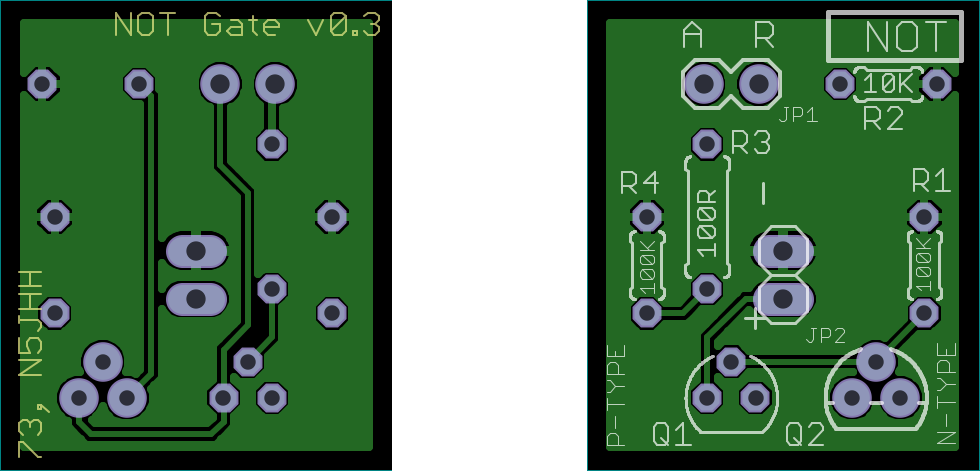
\includegraphics[scale=0.25]{trimmednotgate.png} % convert NOTgate.png -alpha off -trim  trimmednotgate.png 
\caption{A circuit board designed using the more elegant NOT gate schematic seen in Figure \ref{fig:cmosnot}. This one looks almost exactly like the OR gate and the AND gate, but the wiring is different! Also, it has only one input and one output. The NOT gate takes one \emph{input}, A, and produces one \emph{result}, R.}
\label{fig:notgateboard}
\end{center}
\end{figure}

\begin{table}
\begin{tabular}{lllll}
\hline\\[\negsep]
\textbf{Part} & \textbf{Value} & \textbf{Device} & \textbf{Package} & \textbf{Description} \\[\sep]
\hline\\[\negsep]
JP1  &  Input/Output & Pin header    & 1X02 header     & Standard 2-pin 0.1" header \\[\sep]
JP2  &  $V_{in}$ \& $GND$ & Pin header & 1X02 header     & Standard 2-pin 0.1" header \\[\sep]
Q1   &  BS250       &  BS250         & TO-92-3     & P-type MOSFET transistor \\[\sep]
Q2   &  2N7000      & 2N7000         & TO-92-3     & N-type MOSFET transistor \\[\sep]
R1   &  100K        & Small resistor & 0204/5    & Pull-\emph{down} resistor \\[\sep]
R2   &  1K (1000$\Omega$)         & Small resistor & 0204/5    & Current-limiting resistor \\[\sep]
R3   &  100R (100$\Omega$) & $\frac{1}{4}$-watt resistor & 0207/7 & Current-limiting resistor \\[\sep]
R4   &  100K       & Small resistor & 0204/5    & Pull-\emph{up} resistor \\[\sep]
\hline\\
\end{tabular}

\caption{The list of components needed to solder up the NOT gate seen in Figures \ref{fig:cmosnot} and \ref{fig:notgateboard}.}

\end{table}

\clearpage
\newpage

\section{Complex Logic Gates}

Combining gates is possible to produce more complex circuits that answer different questions, like outputs that tell us if two inputs are ``NOT AND" or ``NOT OR" or ``Exclusively OR". Each of these gates allows new comparisons between two inputs, but each is composed of the fundamental three gates, seen above. There is even an "Exclusive NOT OR" gate, which is how computers determine if two numbers are equal to each other.

\subsection*{The NAND Gate}

A ``NOT-AND", or ``NAND", gate just reverses the value obtained from an AND gate -- so it has the exact opposite truth table. Since a NAND gate just reverses the output of AND, you can put a NOT gate on the result (output) line of an AND gate and make a NAND gate, just like you were using Legos.


\medskip
\begin{center}

\begin{tabular}{p{2.3in} p{3.7in} }
\hline\\[\negsep]

The symbol for a NAND gate is:

\vspace{0.25in}

\begin{circuitikz}
	\draw(0,0)
	node[american nand port](nandgate){}
	(andgate.in 1) node [left](){{\color{red}$INPUT~A$}}
	(andgate.in 2) node [left](){{\color{red}$INPUT~B$}}
	(andgate.out) node [right](){{\color{red}$OUT$}};

\end{circuitikz}

\vspace{0.15in}

(see the circle on the output? That's the \emph{not} part)

&

\centering

The ``Truth Table" (how they behave) is: 
\vspace{0.15in}

\begin{tabular}{ll | c}
\multicolumn{3}{c}{\textbf{NAND Gate }}\\
\multicolumn{3}{c}{\textbf{Truth Table}}\\
\hline\\[\negsep]
\textbf{A} & \textbf{B} & \textbf{OUT}\\
\hline
0 & 0 & 1  \\
1 & 0 & 1  \\
0 & 1 & 1  \\
1 & 1 & 0  \\
\hline
\end{tabular}
\\
\tabularnewline

\hline\\[\negsep]

\end{tabular}
\end{center}

\bigskip




\begin{figure}[!h]
\begin{center}
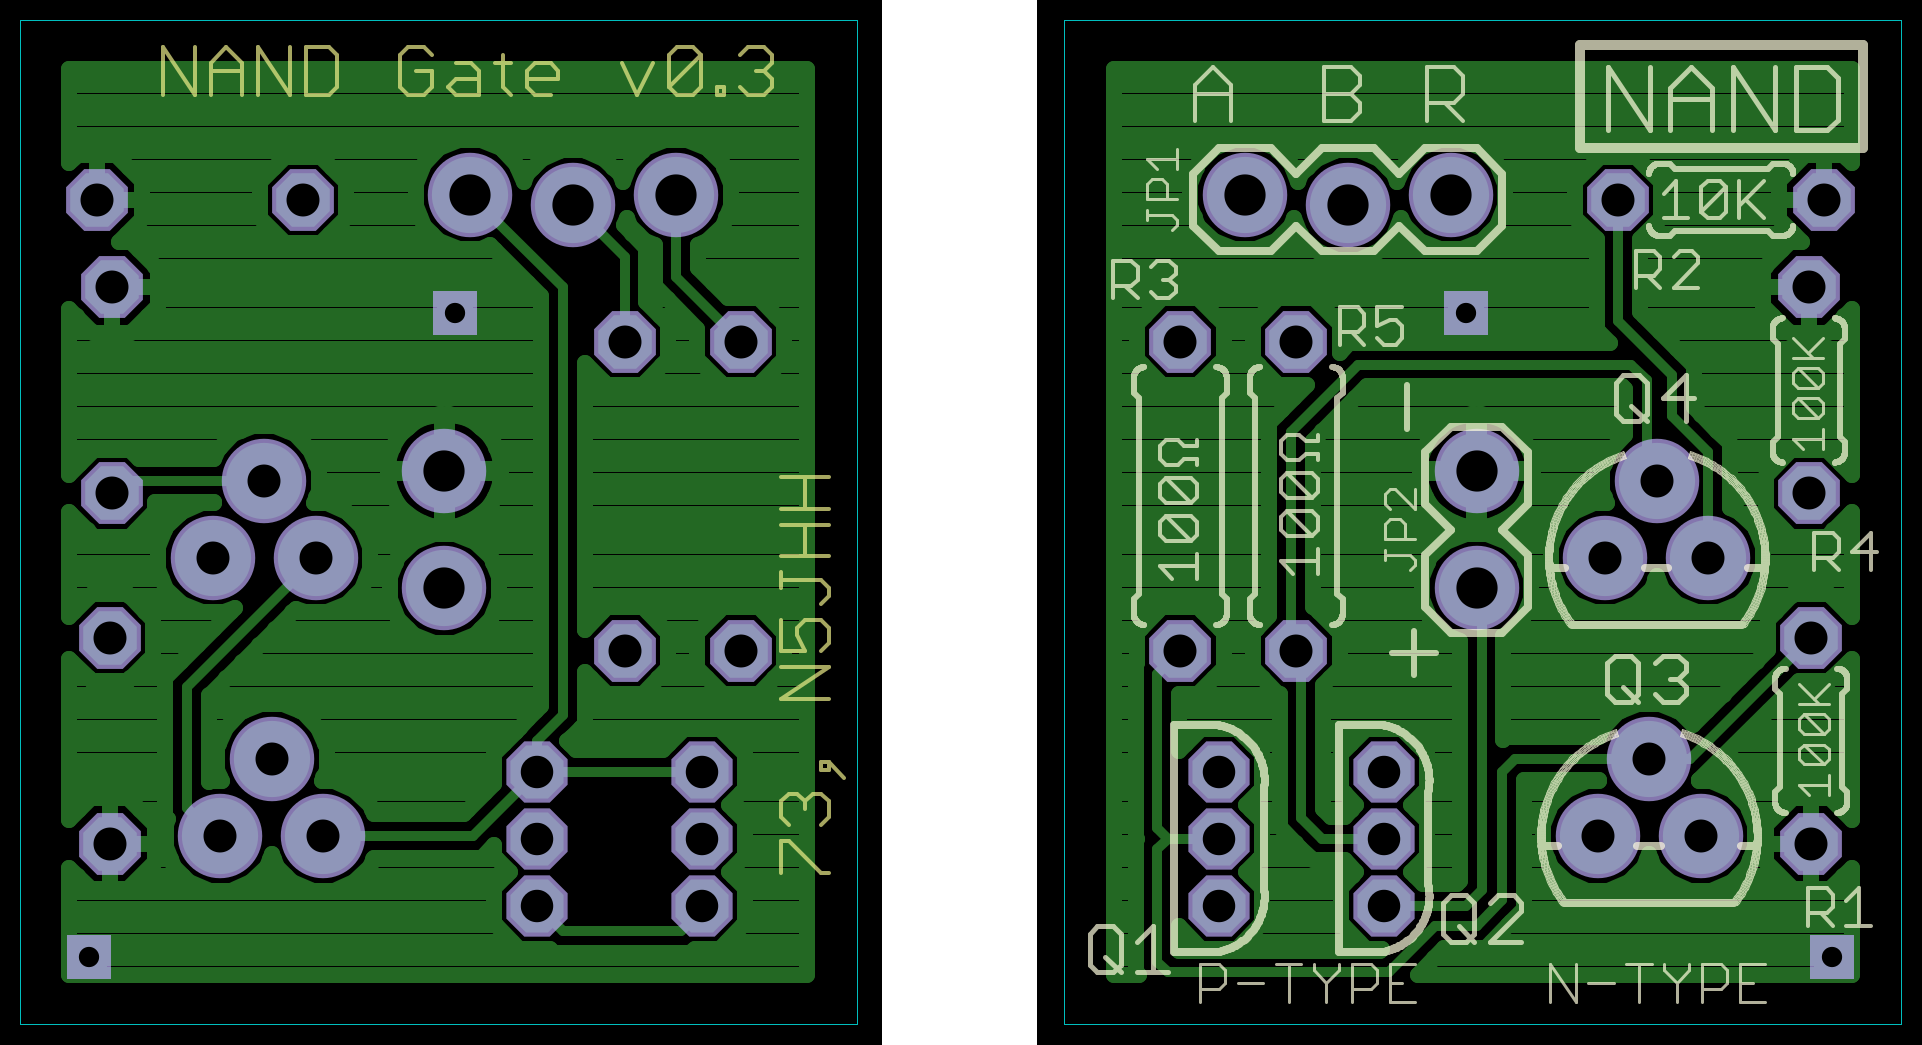
\includegraphics[scale=0.16]{trimmednandgate.png}
\caption{A circuit board designed to make a NAND gate. Note that it uses four transistors.}
\label{fig:nandgate}
\end{center}
\end{figure}

\clearpage
\newpage

\subsection*{The NOR Gate}

Not surprisingly, there is also a NOR gate, that has the reverse truth table to an OR gate. NOR gates are easy to implement, though as we have said elsewhere, more complicated NOR gates save power. 

\medskip
\begin{center}

\begin{tabular}{p{2.3in} p{3.7in} }
\hline\\[\negsep]

The symbol for a NOR gate is:

\vspace{0.25in}

\begin{circuitikz}
	\draw(0,0)
	node[american nor port](norgate){}
	(andgate.in 1) node [left](){{\color{red}$INPUT~A$}}
	(andgate.in 2) node [left](){{\color{red}$INPUT~B$}}
	(andgate.out) node [right](){{\color{red}$OUT$}};

\end{circuitikz}

\vspace{0.15in}

(see the circle on the output? That's the \emph{not} part)

&

\centering

The ``Truth Table" (how they behave) is: 
\vspace{0.15in}

\begin{tabular}{ll | c}
\multicolumn{3}{c}{\textbf{NOR Gate }}\\
\multicolumn{3}{c}{\textbf{Truth Table}}\\
\hline\\[\negsep]
\textbf{A} & \textbf{B} & \textbf{OUT}\\
\hline
0 & 0 & 1  \\
1 & 0 & 0  \\
0 & 1 & 0  \\
1 & 1 & 0  \\
\hline
\end{tabular}
\\
\tabularnewline

\hline\\[\negsep]

\end{tabular}
\end{center}

\bigskip


\begin{figure}[!hb]
\begin{center}
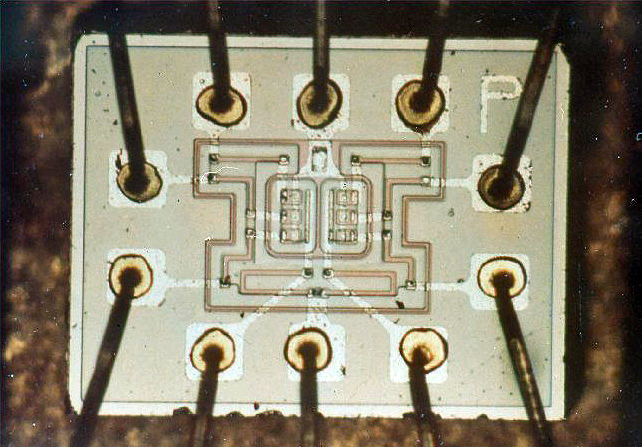
\includegraphics[scale=0.5]{Agc_nor2.jpg}
\caption{An early integrated circuit NOR gate. It has six transistors, eight resistors, and three pairs of A/B inputs (thus, it has three separate yes/no outputs). This chip was part of the guidance computer that took Americans to the moon in 1969. \emph{Photo credit: Wikimedia Foundation}.}
\end{center}
\label{fig:apollonorgate}
\end{figure}


\clearpage
\newpage

\subsection*{The Exclusive-OR Gate}
There is also the ``eXclusive-OR", or ``XOR", gate. The XOR gate output (result) is 1 when \emph{the inputs are not the same}. It returns a 1 if, and \emph{only} if, both inputs are different. That is, it provides a one ``exclusively if'' there is a single ``one'' (sometimes called ``logic high", for ``voltage above zero") in the two inputs. XOR gates take a lot of transistors to implement. The most common version requires 12, though it is possible to make an XOR gate with 8 transistors. See Figure \ref{fig:xorgate}.

\medskip
\begin{center}

\begin{tabular}{p{2.3in} p{3.7in} }
\hline\\[\negsep]

The symbol for an XOR gate is:

\vspace{0.25in}

\begin{circuitikz}
	\draw(0,0)
	node[american xor port](xorgate){}
	(andgate.in 1) node [left](){{\color{red}$INPUT~A$}}
	(andgate.in 2) node [left](){{\color{red}$INPUT~B$}}
	(andgate.out) node [right](){{\color{red}$OUT$}};

\end{circuitikz}

\vspace{0.15in}

(the curved line behind the OR gate means that it is ``exclusive")

&

\centering

The ``Truth Table" (how they behave) is: 
\vspace{0.15in}

\begin{tabular}{ll | c}
\multicolumn{3}{c}{\textbf{XOR Gate }}\\
\multicolumn{3}{c}{\textbf{Truth Table}}\\
\hline\\[\negsep]
\textbf{A} & \textbf{B} & \textbf{OUT}\\
\hline
0 & 0 & 0  \\
1 & 0 & 1  \\
0 & 1 & 1  \\
1 & 1 & 0  \\
\hline
\end{tabular}
\\
\tabularnewline

\hline\\[\negsep]

\end{tabular}
\end{center}

\bigskip

\begin{figure}[!hb]
\begin{center}
\fbox{
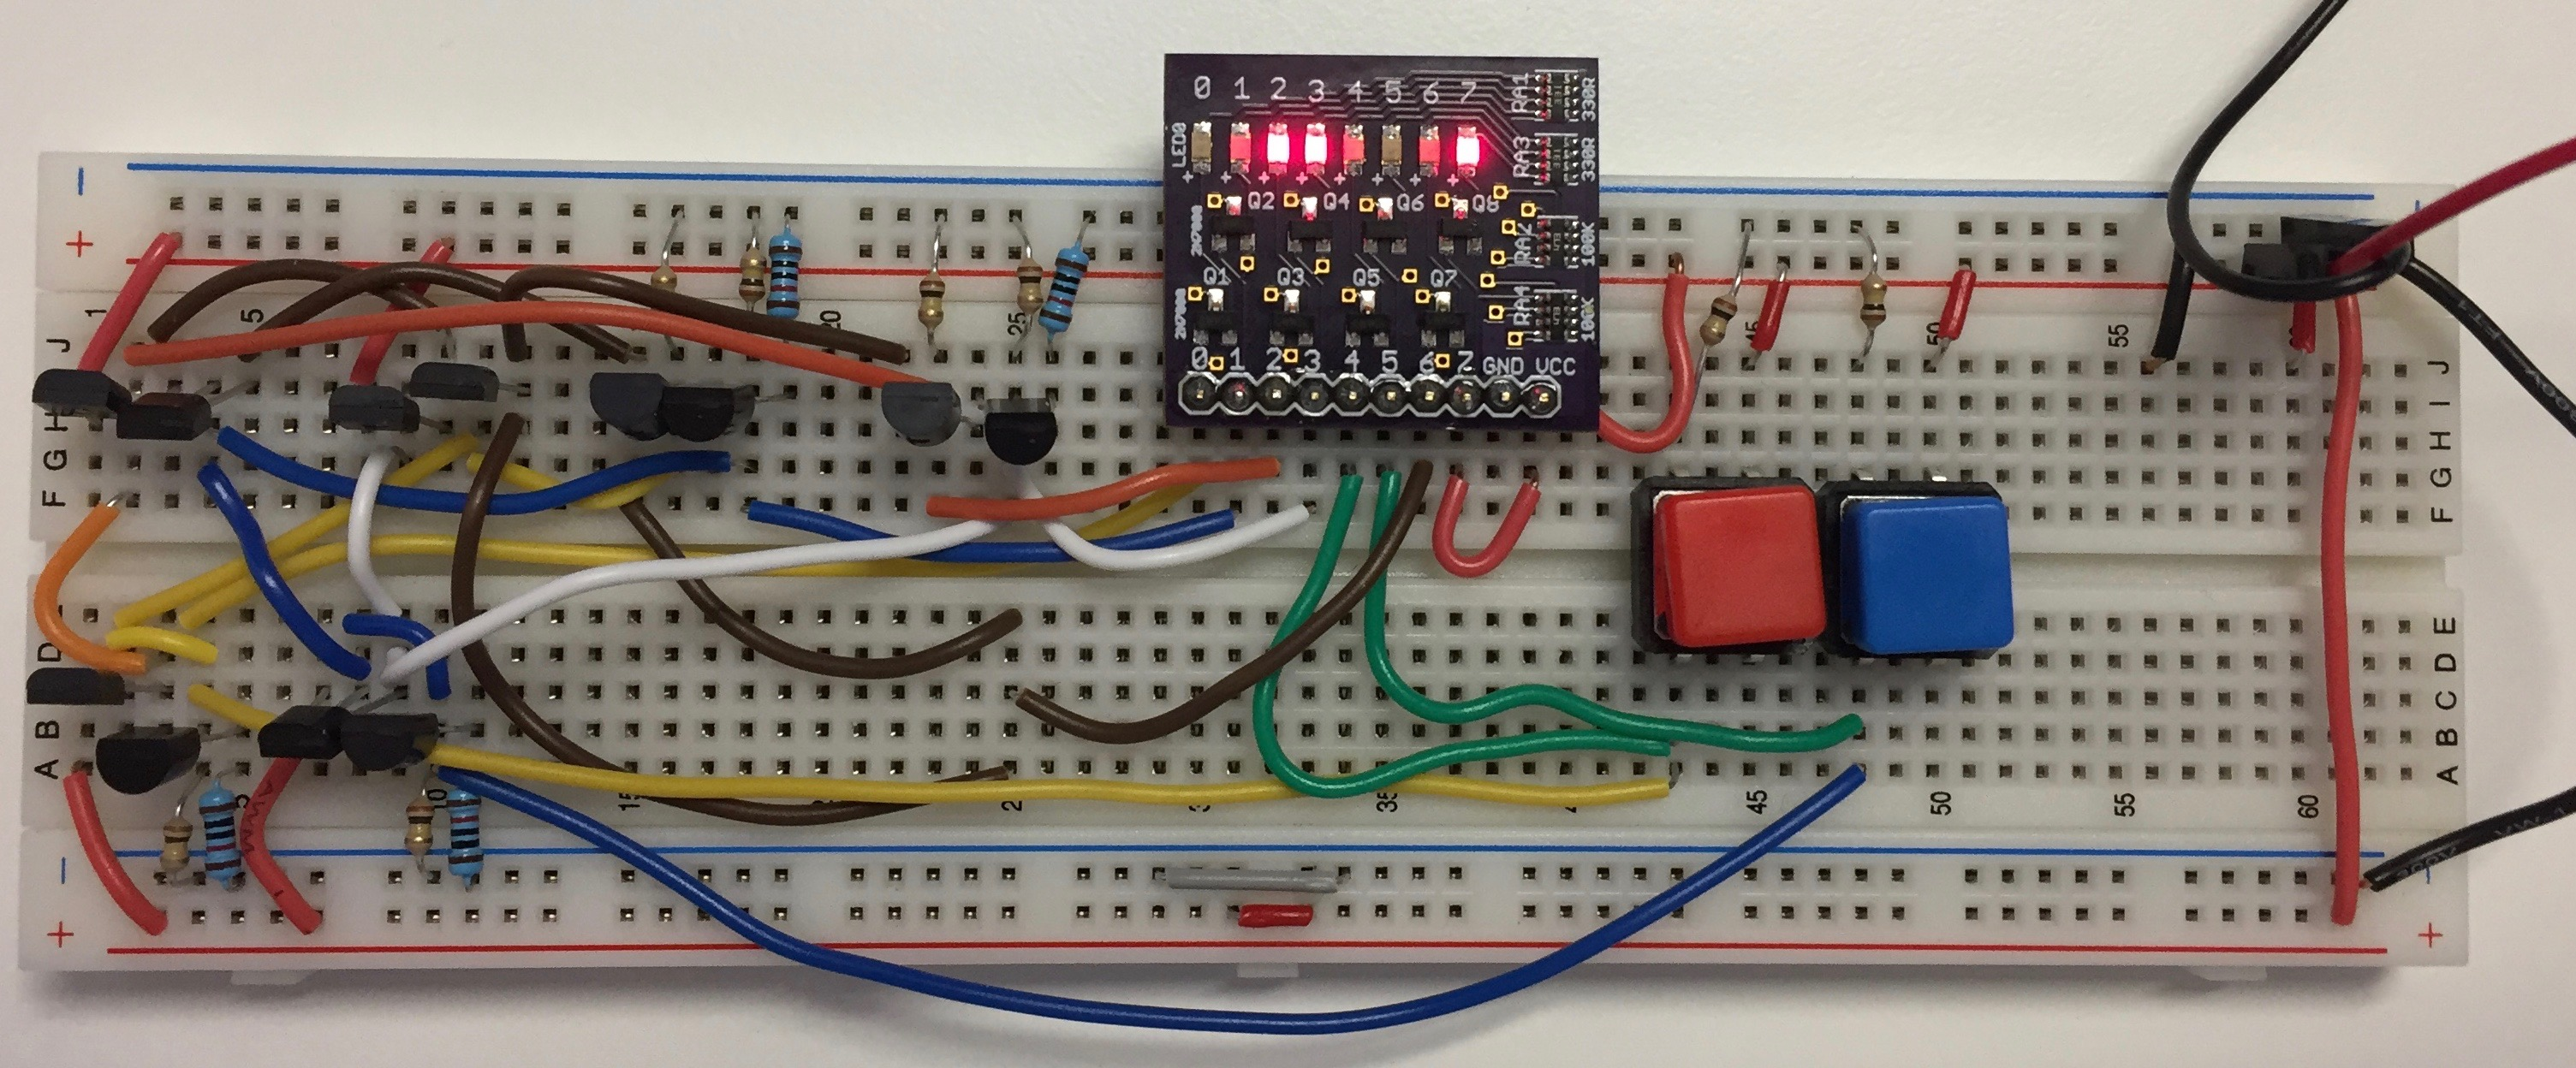
\includegraphics[scale=0.15]{xorgatebreadboard.jpg}
}
\caption{An XOR gate wired up on a breadboard with discrete transistors and resistors. This is the same schematic (and the same color-coded signal wires) seen in Figure \ref{fig:xorgate}. The red switch is signal A and the blue switch is signal B. On the LED line, 0 and 1 are A and B, and 2 and 3 (lit up) are NOT A and NOT B.}
\label{fig:xorbreadboard}
\end{center}
\end{figure}


\begin{figure}[ht!]
\begin{center}
\def\y{8}
\def\x{9}

\begin{circuitikz}

% First NOT gate, Input A
\draw 
	(0,\y+5) node[ocirc](ain) {} % IN node
	(0,\y+5) node[above] {{\color{red}$A$}} % A  label
	
%	(6.75,\y+4) node[short](aout){} % OUT node
	(7,\y+4) node[above] {{\color{red}$A'$}} % NOT A label
	(5,\y+4) |- (6.75,\y+4)
	(5,\y+4) node[circ](){}
	(3,\y+3) node[circ](){}

% Vdd:
	(5,\y+6) node[vcc](avin){}
    (4.5,\y+6) node[above] {$V_{in}$} % Vin

% GND
    (5,\y) node[ground](aground){}
%   (7.75,0.5) node[below] {{\color{red}$GND$}} % GND

% P-type FET
	(5,\y+5) node[pmos, emptycircle, xscale=1](Q1){}
	(5.5,\y+5) node[above]{$Q_1$}

% N-type FET
	(5,\y+3) node[nmos, rotate=0](Q2){}
	(5.5,\y+2.5) node[above]{$Q_2$}

% Resistors:
	(3,\y+3) to [R, l^=$R_1$](3,\y)
	(Q2.S) to [R, -*, l^=$R_2$](aground) 
	(ain) to [R, -*, l^=$R_3$](3,\y+5)

% nets:
	(avin) |- (Q1.S)
	(Q1.D) -* (Q2.D)
	(3,\y) |- (aground)
	(3,\y+5) |- (Q2.G)
	(3,\y+5) |- (Q1.G)

;

% Second NOT gate, Input B
\draw 
	(0,5) node[ocirc](in) {} % IN node
	(0,5) node[above] {{\color{red}$B$}} % B label
	
	(6.5,4) node[circ](notb){} % OUT node
	(6.25,4) node[above] {{\color{red}$B'$}} % NOT B label
	(5,4) |- (notb)
	(5,4) node[circ](){}

% Vdd:
	(5,6.0) node[vcc](vin){}
    (4.5,6.0) node[above] {$V_{in}$} % Vin

% GND
    (5,0) node[ground](ground){}
%   (7.75,0.5) node[below] {{\color{red}$GND$}} % GND

% P-type FET
	(5,5) node[pmos, emptycircle, xscale=1](Q3){}
	(5.5,5.0) node[above]{$Q_3$}

% N-type FET
	(5,3) node[nmos, rotate=0](Q4){}
	(5.5,2.5) node[above]{$Q_4$}

% Resistors:
	(3,3) to [R, l^=$R_4$](3,0)
	(Q4.S) to [R, -*, l^=$R_5$](ground) 
	(in) to [R, -*, l^=$R_6$](3,5)

% nets:
	(vin) |- (Q3.S)
	(3,3) |- (3,5)
	(3,3) node[circ](){}	
	(Q3.D) |- (Q4.D)
	(3,0) |- (ground)
	(3,3) |- (Q4.G)
	(3,5) |- (Q3.G)
;


\draw
% P-type FET
	(\x,\y+5) node[pmos, emptycircle, xscale=1](Q5){}
	(\x+0.5,\y+5) node[above]{$Q_5$}

% P-type FET
	(\x,\y+3) node[pmos, emptycircle, xscale=1](Q6){}
	(\x+0.5,\y+3) node[above]{$Q_6$}

% P-type FET
	(\x+3,\y+5) node[pmos, emptycircle, xscale=1](Q7){}
	(\x+3.5,\y+5) node[above]{$Q_7$}

% P-type FET
	(\x+3,\y+3) node[pmos, emptycircle, xscale=1](Q8){}
	(\x+3.5,\y+3) node[above]{$Q_8$}

% Vdd:
	(\x,\y+6) node[vcc](cvin){}
    (\x+0.5,\y+6) node[above] {$V_{in}$} % Vin

% Vdd:
	(\x+3,\y+6) node[vcc](dvin){}
    (\x+3.5,\y+6) node[above] {$V_{in}$} % Vin

% Nets:
	(Q5.D) to (Q6.S)
	(Q7.D) to (Q8.S)
	(cvin) to (Q5.S)
	(dvin) to (Q7.S)
;


\draw
% N-type FET
	(\x,\y-1) node[nmos, xscale=1](Q9){}
	(\x+0.5,\y-1) node[above]{$Q_9$}

% N-type FET
	(\x,\y-3) node[nmos, xscale=1](Q10){}
	(\x+0.5,\y-3) node[above]{$Q_{10}$}

% N-type FET
	(\x+3,\y-1) node[nmos,  xscale=1](Q11){}
	(\x+3.5,\y-1) node[above]{$Q_{11}$}

% N-type FET
	(\x+3,\y-3) node[nmos, xscale=1](Q12){}
	(\x+3.5,\y-3) node[above]{$Q_{12}$}

% Grounds:
    (\x,2) node[ground](ground2){}
    (\x+5,-1) node[ground](ground3){}

% Current-limiting resistors:
	(Q10.S) to [R, -, l^=$R_7$](ground2) 
	(Q12.S) to [R, -, l^=$R_8$](12,2) 
	
% Nets:
	(Q11.S) to (Q12.D)
	(Q9.S) to (Q10.D)
	
	(Q8.D) to (Q11.D)
	(Q6.D) to (Q9.D)
	
	(\x, \y+4.0) -| (\x+3, \y+4.0)	
	(\x,\y+4.0) node[circ](){}
	(\x+3,\y+4.0) node[circ](){}

	(12,2) -- (14,2) -- (ground3)

;

% A signal:
\draw[ultra thick, yellow]
	(3,\y+5) -- (3, \y+7) -- (6, \y+7) -- (6,\y-1) -- (Q9.G)
	(6,\y+5) node[circ, color=yellow](){}
	(6,\y+5) -| (Q5.G)
;


% B signal:
\draw[thick, blue]
	(3,4) -| (2, 4) -- (2, -1) -| (7,-1) -- (7,5) --  (7.5,5) -- (Q10.G)
	(3,4) node[circ, color=blue](){}
	(7.5,5) node[circ, color=blue](){}
	(7.5,5) -- (7.5,10) --  (10,10) -- (10,13) -- (Q7.G)
;


% NOT A signal:
\draw[thick, orange]
	(6.75,\y+4) -- (7.25, 12) -- (7.25, -1.0) -- (10.5, -1.0) -- (10.5,7) -- (Q11.G)
	(7.25,11) -- (Q6.G)
	(7.25,11) node[circ, color=orange](){}
	(6.75,\y+4) -- (5,\y+4)
;


% NOT B signal:
\draw[line width=3, color=black]
	(5,4) -- (6.5, 4) -| (6.5, 0.5) -- (10,0.5) -- (10,5) -- (Q12.G)
	(10,3) -- (10,8.0) -- (11, 8.0) -- (Q8.G)
;

\draw[thick, color=white]
	(5,4) -- (6.5,4) --  (6.5,0.5) -- (10,0.5) -- (10,5) -- (Q12.G)
	(10,3) -- (10,8.0) -- (11, 8.0) -- (Q8.G)
;

%\draw
%	(6.5, 4) node[circ, color=black](){}
% ;

\draw
% Pull-down resistors, R9 (NOT_A) and R10 (NOT_B)
	(10.5,-1.0) node[circ, color=orange](){}
	(10.5,-1.0) to [R, -* , l^=$R_9$](14,-1)

	(10.0,0.5) node[circ, color=black](){}
	(10.0,0.5) to [R, -* , l^=$R_{10}$](14,0.5)


;

% XOR signal:

\draw[color=brown, ultra thick]
	(\x, \y+1) -* (\x+3, \y+1)
	(\x,\y+1) node[circ](){}
	(\x+3,\y+1) node[circ](){}
	
	(\x+5,\y+1) node[circ](xor){} % OUT node
	(\x+4.25,\y+1) node[above] {{\color{red}$A~XOR~B$}} % XOR label
	(\x+3,\y+1) |- (xor)
;

% Labeling and explanation
\draw
 (15,6) node[align=left](exp1){This pair of AND \\ gates grounds \\ the circuit if \\ both inputs are \\  the same.}

 (15,12) node[align=left](exp1){This pair of AND \\ gates controls \\ circuit power input. \\ Each (linked) pair \\ only functions if the \\ inputs are different.}

 (1,7) node[align=left](exp1){Two NOT \\ gates enable \\ comparisons \\ among inputs.}

;


\end{circuitikz}

\caption{An exclusive-or (XOR) gate, composed of 12 transistors and some supporting resistors. You don't need to understand how it works, but it's not that hard if you break it down into the colored signals, two NOT gates, two AND gates with N-type FETs, and two linked AND gates with P-type FETs. A ``0'' signal opens a P-type FET, and a ``1'' signal opens an N-type FET.}
\label{fig:xorgate}
\end{center}
\end{figure}

\clearpage

